\section{Methods, Tools and Frameworks}
% In this section, you should describe the methods, programming languages, packages, tools and framework you plan to use.
% for this report, you can list some you have identified and intend to use.
% No need to give any details.     

\subsection{Tools}
\todo[inline]{Is this section ``tools'' or ``Methods'' or ``Frameworks''??}
\subsubsection{Chatbot GUI}
\begin{itemize}
    \item Graphical User Interface: GUI development using JS, NodeJS, HTML, CSS.
    \item Voice Commands: Text-to-Speech \& Speech-To-Text recognition using APIs such as webkitSpeechRecognition, SpeechRecognition etc. 
\end{itemize}
\subsubsection{Web Scraping}
\begin{itemize}
    \item Selenium: This library will be used to scrape data from the wesbites who doesn't provide any API to extract data in form of response.
    \item Requests: This module will be used to extract data via HTTP/HTTPS requests.
    \item BeautifulSoup: This library will be used to scrape wesbites HTML elements to fetch data.
\end{itemize}
\subsubsection{Chatbot Conversation - NLP}\label{Sec: Methods/NLP}
    \begin{itemize}
        \item Spacy: This library will be used for natural language processing specifically for named-entity recognition (NER).
        \item Nltk: This toolkit will be used along with spaCy for NLP.
        \item Fuzzywuzzy: This library will be used to determine closes matches in the user input to extract relevant information.
        \item Experta: This library will be used for building expert systems to provide suitable answers to the user.
    \end{itemize}

\subsubsection{Regression Model Prediction}
\paragraph{Models Utilised}
A variety of commonly implemented regression models were employed to predict the arrival at Norwich from the departure from London Liverpool Street. These models incline:
\begin{itemize}
    \item Multi Layer Perception (MLP) Regression: the sklearn.neural\_network library will be used to build a simple MLP model \citep{scikit-learn}.
    \item K-Nearest Neighbors (KNN) Regression: the sklearn.neighbors library will be used to build and tune a K-Nearest Neighbors model \citep{scikit-learn}.
    \item XGBoost (XGB) Regression: the XGBoost model from \cite{chen2016xgboost} will be implemented.
    \item Random Forest (RF) Regression: the sklearn.ensemble library will be used to build and tune a Random Forest model \citep{scikit-learn}.
    \item Linear Regression: the sklearn.linear\_model library will be used to implement a Linear Regression model \citep{scikit-learn}.
    \item Huber Regressor: the sklearn.linear\_model library will be used to implement a Huber Regressor model \citep{scikit-learn}.
    \item Lasso Regressor: the sklearn.linear\_model library will be used to implement a Lasso Regressor model \citep{scikit-learn}.
    \item Stochastic Gradient Descent Regressor: the sklearn.linear\_model library will be used to implement a Stochastic Gradient Descent Regression model \citep{scikit-learn}.
\end{itemize}

\paragraph{Metrics and performance evaluation}\label{Sec: Regression Metrics & performance}
During the training process each model will be fitted to 80\% of the dataset while 20\% will be employed as validation data. Each model will predict the arrival time at Norwich based on the values in the training dataset.

    \begin{itemize}
        % \item Sklearn neural\_network: is used the build a very basic MLP before a Keras model
        % \item sklearn.neighbors\_KNeighborsRegressor: Is used as a basic KNeighborsRegressor model
        % \item Tensorflow: Keras id the foundation of the neural network model.
        % \item Tensorboard: This utility extension for Tensorflow library was be used to visualise the model metrics.
        \item NumPy: This was used for data manipulation and numerical calculate \citep{harris2020array}.
        \item Pandas: This was used for data storage inside dataframes along with dataframe manipulation tasks \citep{reback2020pandas}.
        \item sklearn: This library was used for data preprocessing and model metrics \citep{scikit-learn}.
        \item Seaborn and MatPlotlib: was used to generate visual representation of the data \citep{Waskom2021},\citep{Hunter:2007}.
    \end{itemize}

% You may list some methods you will use for developing your chatbot, including 
   
% Such as what type of user interface (graphical, text, or voice, etc) you intend to use.

% What Natural Language Processing and understanding methods you intend use, 

% What referring or reasoning methods

% What prediction methods, such as kNN, neural networks etc. 

% \todo{Change this to a better diagrame | Move to different section}
% \begin{figure}
%     \centering
%     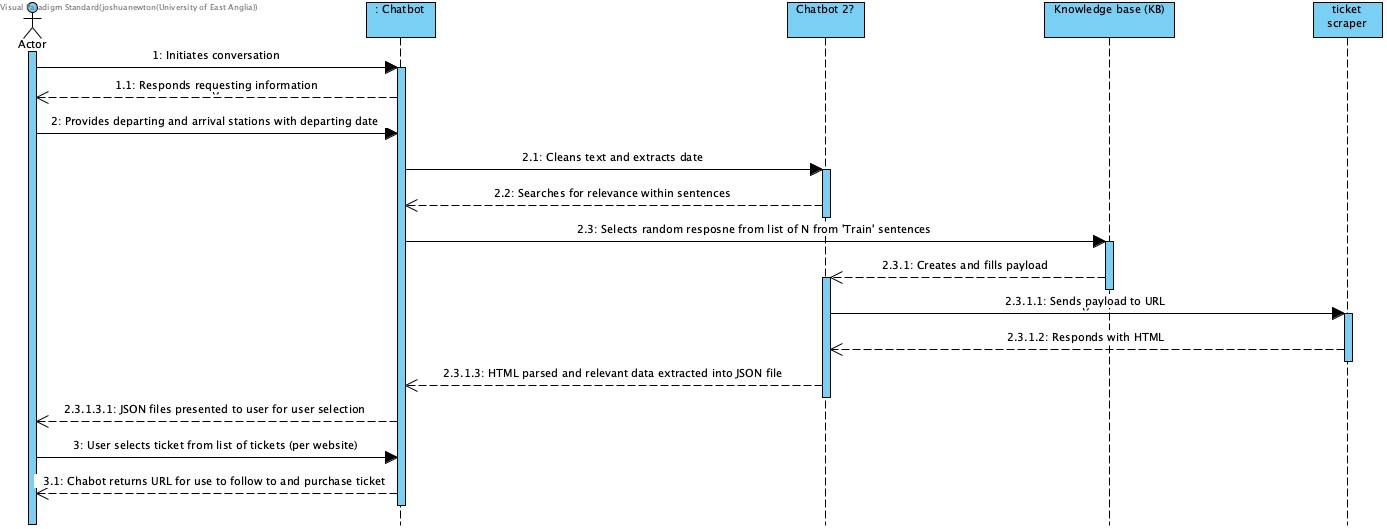
\includegraphics[width= \textwidth]{Diagrams/AI_Assign_02-Seq_Diag_01.jpg}
%     \caption{High level view of current chatbot response and web scraping system}
%     \label{fig:enter-label}
% \end{figure}

             
\subsection{Languages, Packages, Tools}
The primary programming languages used for this project are Python and JavaScript.
Postgres will be considered for the database should a database be required. The project has found sufficient success using local csv files as an alternative to databases.

\paragraph{Programming Languages:} Python, JavaScript, or others.
\paragraph{GUI development:} using HTML \& CSS 
\paragraph{Packages:} NLP, NLTK locationtagger\citep{NLTK}, Spacy's ``en\_core\_web\_lg model''. For matching regex patterns: Selenium, requests, html-requests, BeautifulSoup, Minidom, lxml, urllib3 etc\dots %for web scraping mechanism. 
\paragraph{KnowledgeBase and Engine:} PyKE, PyKnow, Experta, or others. 
% \paragraph{Database:} Postgres, or MongoDB
 
\subsection{Development Framework}
The following sections outline and describe the current efforts and developments made towards achieving the aims and objectives described in Section \ref{Sec: Aim and Objs}.

\subsubsection{Flowchart}
Figure \ref{Fig: Flowchart} details a high-level flow chart of the chatbot when the user requests a train ticket. 

\subsubsection{Use Case and Sequence Diagrams}
Figure \ref{Fig: use case whole system} describes a use case diagram of the whole system. Also the general logic of the Chat-bot constructed by following the algorithms of the sequence diagrams which are stated in figure \ref{}, \ref{}, and \ref{} for each of the parts.

% \begin{figure}[!htbp]
%     \centering
%     \includegraphics[width=0.8\linewidth]{Diagrams/USECASEfull_system.png}
%     \caption{A high-level Use case Diagram of the Chat Bot}
%     \label{Fig: User-case_whole Diagram}
% \end{figure}

% \begin{figure}[!htbp]
%     \centering
%     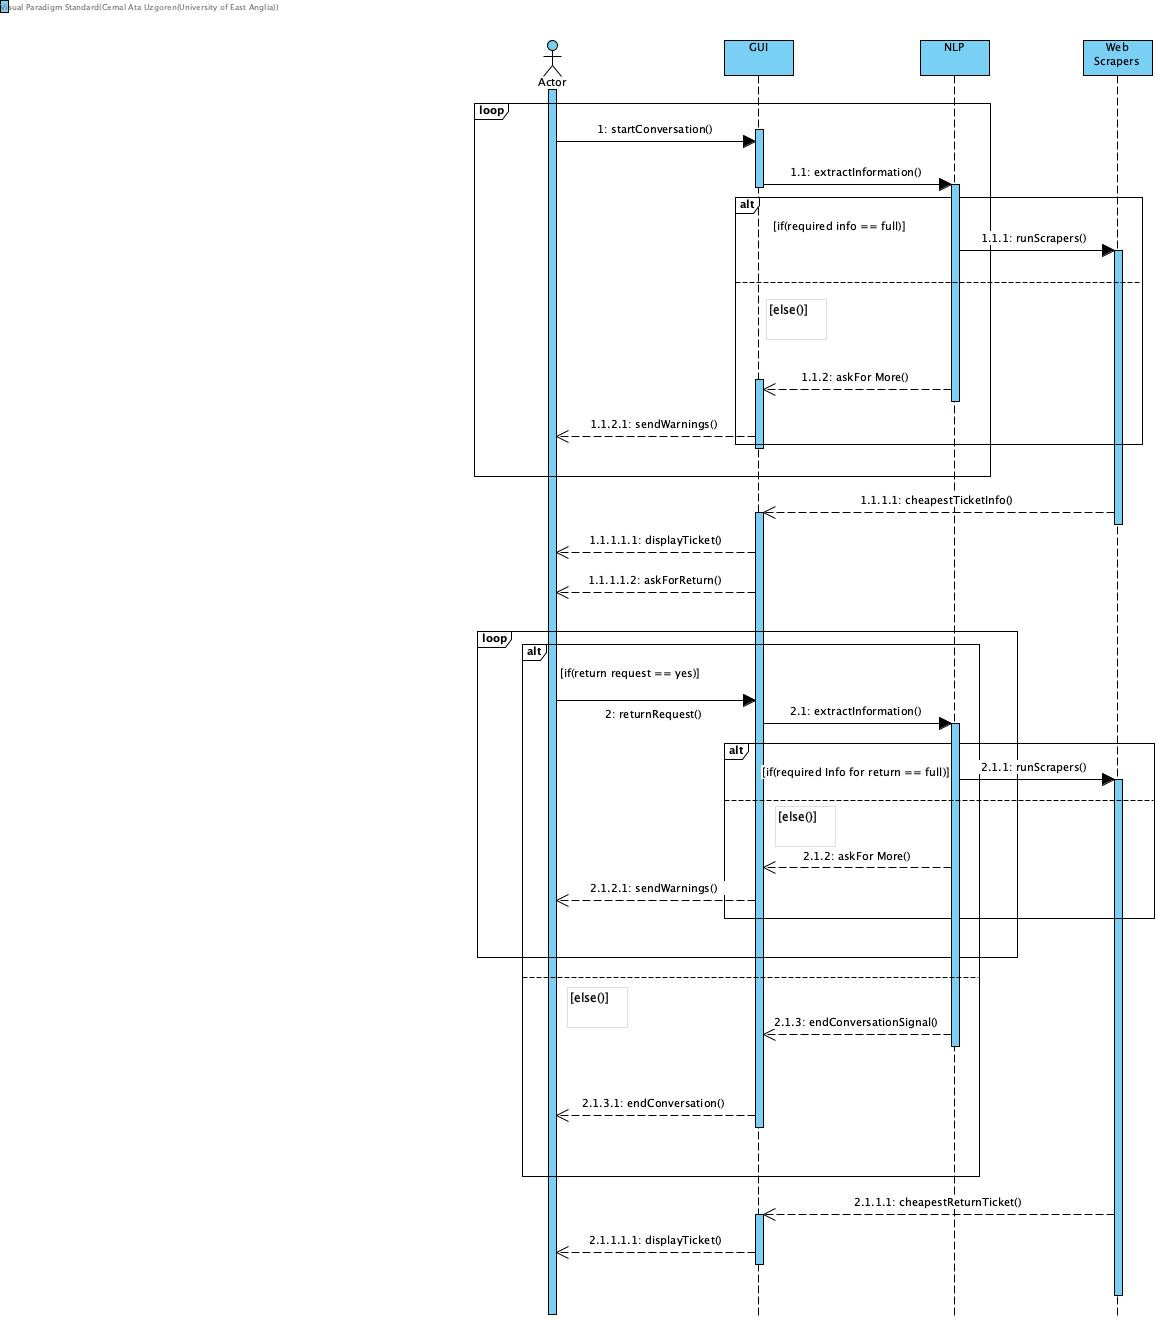
\includegraphics[width=0.8\linewidth]{Diagrams/Sequence Diagram of Part-1.jpg}
%     \caption{Sequence diagram of the Part 1}
%     \label{Fig: part_1_sequence}
% \end{figure}

% \begin{figure}[!htbp]
%     \centering
%     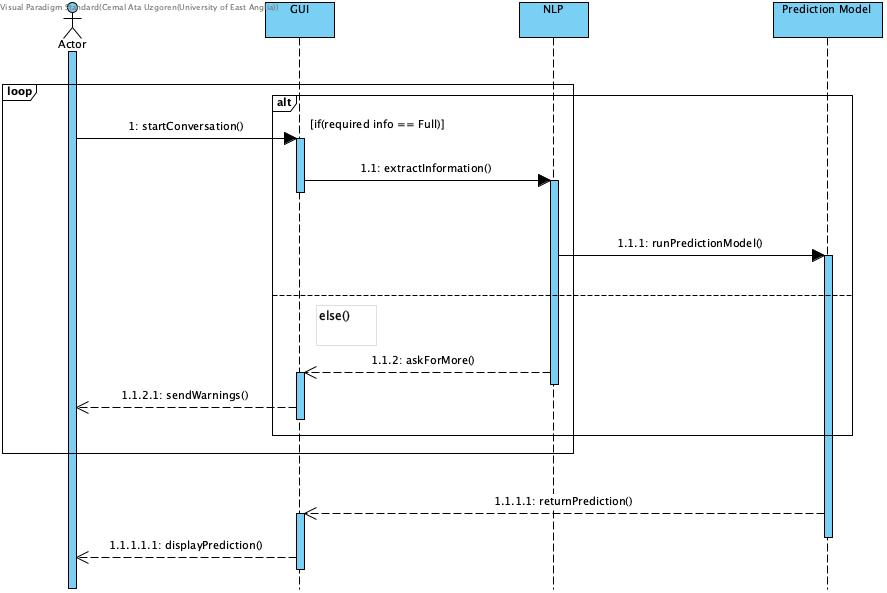
\includegraphics[width=0.8\linewidth]{Diagrams/Sequence Diagram of Part-2.jpg}
%     \caption{Sequence diagram of the Part 2}
%     \label{Fig: part_2_sequence}
% \end{figure}

% \begin{figure}[!htbp]
%     \centering
%     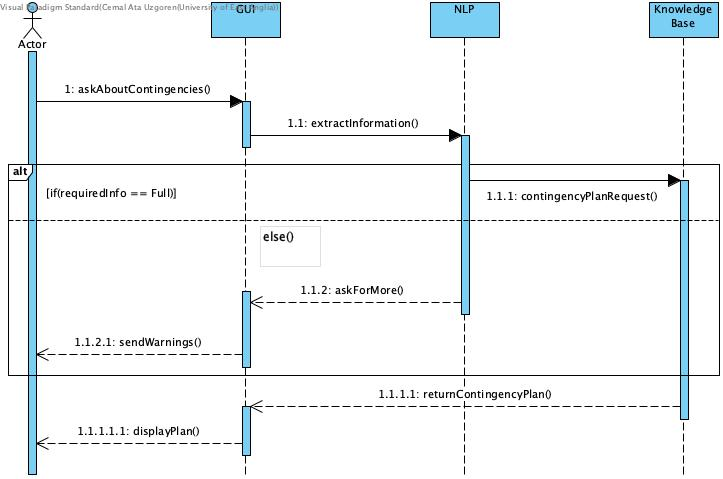
\includegraphics[width=0.8\linewidth]{Diagrams/Sequence Diagram for Part-3.jpg}
%     \caption{Sequence diagram of the Part 3}
%     \label{Fig: part_3_sequence}
% \end{figure}

\subsubsection{Sequence Diagrams}\label{Sec: Sequence Diagrams}
The following sections will describe the sequence diagrams for each mechanism the acheive the goals outlined in Section \ref{Sec: Aim and Objs}.
\subsubsection*{Ticket Scraping Mechanism}
Figure \ref{Fig: seq diag ticket scraping} shows the sequence diagrams which involves a structured sequence of interactions between the user (actor), graphical user interface (GUI), natural language processing (NLP) system, and web scrapers. The process begins when the user initiates a conversation via the GUI, which then requests the NLP system to extract information from the user's input. If the information provided is incomplete, the system prompts the user for additional details. Once complete information is obtained, the NLP system activates web scrapers to retrieve the cheapest available ticket details, which are then displayed to the user.\vspace{0.5cm}

\noindent
If the user requests a return ticket, the system processes this similarly by extracting the necessary return trip information and verifying its completeness. Incomplete information prompts further user queries. Upon obtaining complete return information, the NLP system runs the web scrapers to find the cheapest return ticket, which is subsequently presented to the user.\vspace{0.5cm}

\noindent
Throughout the interaction, the system may send warnings to keep the user informed of any issues or important notices. The conversation concludes once the user's inquiries are fully addressed, with the system ending the interaction through predefined methods. This model ensures efficient and accurate handling of ticket inquiries by leveraging robust communication between the user, GUI, NLP system, and web scrapers.

\subsubsection*{Delayed Arrival Prediction}
Figure \ref{Fig: seq diag delay prediction} details the sequence diagram when the chatbot is utilising the regression model. The process is initiated when the actor starts the conversation. Subsequently, the system performs a completeness check on the required information. If all necessary data is available, the system extracts the relevant details and executes the prediction model. The resultant prediction is then presented to the user through the display function. However, if the system encounters insufficient information, it prompts the user for additional input. Additionally, the system may issue warnings to alert the user of any potential issues.

\subsubsection*{Contingency Plan}
Figure \ref{Fig: seq diag contingency} depicts how the actor interacts with the chatbot to be advised on what contingency to follow in an unexpected event or emergency. The sequence starts with the actor invoking a conversation about contingencies. This function then calls the extracts the relevant information from the prompt, which gathers information about the contingency plan from the knowledge base. Following this, there is an alternate decision point, the decision is made based on whether the required information is filled enough to be satisfactory.
If the ``requiredInfo'' is filled, then the a function is called to request the corresponding contingency plan. This function retrieves the complete contingency plan from the knowledge base. Finally the function will finally present the corresponding plan to the user. On the other hand, if the required info does not contain enough information, then a function is invoked to prompt the actor to insert the required information the missing fields through short warnings.

\subsubsection{Graphical User Interface Development}
The graphical user interface (GUI) is developed with text-to-speech and speech-to-text recognition feature embedded. The interface understands the voice commands given by user and displays on the UI. Based on the commands received, it attempts to fetch the result from the NLP and displays back on the screen. A spinner / loader is also implemented while the response is being fetched by chatbot for a reliable experience. Figure \ref{Fig: GUI Example} shows an example of the current GUI state.

\subsubsection{NLP Implementation}
The development of the natural language processing (NLP) behind the chatbot was made using a combination of SpaCy, NLTK (Natural Language Tool Kit), Scikit-learn and other in-built python libraries. The user input sentence was lemmatised first, meaning  linking similar meaning words as one word \cite{lemmatization}, then extracting the relevant details to fulfill the task and finally performing action as per the detected task and providing the appropriate response back to the user. \paragraph{Lemmatization:} The stop words were removed during the sentence cleaning process but leaving \textit{to} and \textit{from}. The intention behind leaving these two words were to figure out the origin / departing and arriving stations from the users input. \paragraph{Labels Creations \& Detection:} There were various different labels which were created as per the tasks which this chatbot should be able to perform. Some of the key labels are \textit{train}, \textit{location}, \textit{date}, \textit{time}, \textit{return}, \textit{delay}, \textit{contingency}, \textit{blockage}, \textit{assist}, \textit{help} etc. The sentences matched against these labels invoke their respective functionality functions to perform their tasks to achieve the end goal. \paragraph{Similarity Check:} The sanitised user input gets matched to the label which it belongs. The system calculate the similarity index via \textit{similarity()} which is an in-built function within spaCy python module. If the similarity matches with the minimum similarity defined threshold, it invokes a certain task as per the matched label. \paragraph{Stations Extraction: } It was observed that the spaCy and NLTK in-built functions could only fetch the renowned cities of the UK such as London, Birmingham, Manchester etc but they could not fetch small cities / stations such as Exeter, Norwich, Seven Kings etc. Hence they were not fully reliable and another approach had to be implemented. The \textit{stations.csv} containing all possible stations within the United Kingdom was used to match the stations against the user input. The already lemmatised user input which re-cleansed even more to shrink the user input as much as possible so that the match could have been easy. If there an exact match of the station in the user input to \textit{stations.csv}, the system would return the exact matching stations. Even the input has a partial match in case there is spelling mistake or there is a genuine partial matching for instance, if user enters London as input but London contains 10+ train stations such as London Piccadilly or London Liverpool Street etc, the system would return all the partially matched station asking the user to choose the precise ones. \paragraph{Date \& Time Extraction:} The time extraction was performed mainly using python regex matching. Since spaCy and NLTK libraries performed quite poorly in time extraction from a sanitised sentence, various regex matching were placed instead. \paragraph{Return Ticket Mechanism:} Return ticket functionality has been implemented in the first task of the chatbot that is to find the cheapest train fare within the UK. The chatbot asks the user once one-side train fare search is performed if the user wants to view cheapest return fares as well. The user may wish not to view return fares and simply quit the conversation. But NLP has been implemented if user wishes to view return fares too. Assuming the return would be within the same stations as one-way search, hence the chatbot would ask the user for only date and time of the return. Once the details are provided, the return fares are then searched and returned on the GUI. \paragraph{Delay Calculation Mechanism:} The delay calculation was implemented comprising of the details which are required from the user as input followed by invoking the saved ML model for predicted delay time calculation. The chatbot asks the user for the time of the last or current departed station, the name of the last or current departed station and lastly the time when the user departed from the origin station i.e by default London. Once all the details are received, the chatbot returns the predicted delay to reach to the destination i.e Norwich on it's user interface. \paragraph{Contingency Plans:} The NLP implemented behind the task of providing the contingency plans to the train station staff comprise of the details such has the name of the train stations on the Great Eastern Track in Greater Anglia facing the blockage and the type of the blockage i.e either \textit{Partial} or \textit{Full}. On receiving this information from the user, the alternate plans / routes are displayed on the chatbot GUI.

\paragraph{Web Scraping}
\todo[inline]{Double check the following websites still work! - also add a section about which ones do not work / have changed since development}
The model is developed to extract the required data from the following train booking websites:
\begin{enumerate}
    \item \href{https://www.lner.co.uk/}{LNER}
    \item \href{https://www.greateranglia.co.uk/}{Greater Anglia}
    \item \href{https://www.mytrainticket.co.uk/}{My Train Ticket}
    \item \href{https://www.nationalrail.co.uk/}{National Rail}
    \item \href{https://www.southernrailway.com/}{Southern Railways}
    \item \href{https://www.mytrainpal.com/}{Train Pal}
\end{enumerate}

The required information extracted are as follows:

\begin{itemize}
    \item Chepeast website name
    \item Fare amount
    \item Cheapest fare website link
\end{itemize} 

\subsubsection{Regression Model}
The developments into the delayed arrival time predictive model was made using a combination of JuPyter Notebook and the later integration into the conversational Python script. The Notebook environment was chosen as an intuitive way to display and understand the data processing and model training. Once the model(s) were trained and saved to a recallable file, code to recall each file embedded into Python scripts then become the main executable location.

\paragraph{Data Types}\label{sec: Data Processing}
A detailed review of the data revealed that the majority of value types were string formats with 24-hour time values. Initially, there was a plan to encode each column containing string values using an array of methods including Binary Encoding, One Hot Encoding, Label Encoding, and Target Encoding. However, due to the complexity and quantity of unique values, encoding timestamp values proved inefficient. Instead, the Pandas library was utilised to convert the string value to datetime objects using the format Hour : Minute. Immutable or missing values are handled and replaced with a Not A Time (NaT) value.\vspace{0.5cm}

\noindent
The timecode objects were transformed to calculate the number of seconds since midnight. This calculation involves multiplying the hour component by 3600, the minute component by 60, and summing these products. The reason for using this method is that it provides a simpler normalisation process, simplifies calculations, and reduces dimensionality, which in turn can improve model performance. 

\paragraph{Encoding the tlp}\label{sec: Encoding the tlp}
As described in Table \ref{tab: Table of dataset column headers} the column ``tlp'' held the timing point locations for all stations of the journey. Examples of the values included: ``SHENFLD'', ``NRCHTPJ'', ``NRCH'' and ``TROWSEJ''. Due to the data only containing journeys between London Liverpool Street and Norwich, there were 34 unique values as described in Table \ref{tab: Table of dataset column headers}. Due to to considerably small quantity of values, the Label Encoder method is utilised as the encoder. Table \ref{tab:tpl encoding} showed the original ``tlp'' values and their corresponding encoded values.

\paragraph{Binary Valued Columns}
In addition to the encoding practices described Section \ref{sec: Encoding the tlp},it is important to note that while columns with binary values were encoded with either a ``1'', ``0''. These encoded representations did not feature in the final set of extracted features as they were deemed less effective for our predictive modelling objectives.

\paragraph{Feature Extraction}
The dataset comprised an extensive range of timestamps that incorporated predicted, estimated, planned, and actual times. Table \ref{tab: Table of dataset column headers} outlines the features paired with a description. The essential features necessary to predict arrival time at Norwich (NRW) during a journey from London Liverpool Street (LST), included the station's unique code, the departing time from LDN, departing time from each individual station and arrival time at NRW. As a result of adopting a simple feature set, there was an efficient systematic approach to handling missing values detailed in the following section.

\paragraph{Missing Values}\label{sec: missing values} The dataset contained an inherently large proportion of NaN values owing to a single time value being recoded at a singular point in time. To mitigate the issue of missing data, an systematic strategy was employed that involved the conditional imputation based on temporal availability. The process was structured hierarchically; firstly, the extraction of actual departure and arrival time instances were prioritised; however, when such records were unavailable, estimated values were introduced. Should the estimated values also be null, predicted values were employed as a final resort. As an additional method for dealing with missing information, passing times were occasionally used.